\documentclass[color]{tudbook}
\usepackage[T1]{fontenc}
\usepackage[latin1]{inputenc}

\usepackage{listings}
\usepackage{graphicx}
\usepackage{eso-pic}
\usepackage{pstricks}
\usepackage{listings}
\usepackage{graphicx}
	
\definecolor{darkgreen}{rgb}{0,0.5,0}


% F�r listings
\usepackage{listings}
\lstset{
  frame=single,
  frameround=tttt,
  xleftmargin=0.7cm,
  xrightmargin=0.3cm,
  numbers=left,
  basicstyle=\fontfamily{pcr} \small \color{black},
  keywordstyle=\bfseries \color{blue},
	stringstyle=\color{red},
	commentstyle=\color{darkgreen},
	breaklines=true,
	showstringspaces=false
}

\newcommand{\reference}[1]{{\begin{ttfamily}#1\end{ttfamily}}}
\newcommand{\keyword}[1]{{\begin{itshape}#1\end{itshape}}}
\newcommand{\eclipse}[1]{{\begin{itshape}#1\end{itshape}}}

% Define Faculty and Institute
\einrichtung{Fakult�t Informatik}
\institut{Institute for Software- und Multimediatechnik}
\professur{Lehrstuhl f�r Softwaretechnologie}

% Define the title of the thesis
\title{An Introduction into Dresden OCL2 for Eclipse}
% Specify the author of the thesis
\author{Claas Wilke}
% Specify the date on which the thesis is handed in
\date{Last update: \today}

% F�r Metadaten im PDF.
\usepackage[
  bookmarksnumbered=true,
  pdftitle={An Introduction into Dresden OCL2 for Eclipse},
  pdfauthor={Claas Wilke},
  pdfcreator={TeXnicCenter},
  pdfkeywords={OCL, Dresden OCL, constraints},
  pdfsubject={A Tutorial which introduces into Dresden OCL2 for Eclipse.}
]{hyperref}

\hypersetup{
  colorlinks=true,
  linkcolor=HKS41-100,
  citecolor=HKS41-100,
  filecolor=HKS41-100,
  menucolor=HKS41-100,
  urlcolor=HKS41-100
} 


\begin{document}




\maketitle




\tableofcontents




\chapter{Introduction}

This tutorial generally introduces into \keyword{Dresden OCL2 for Eclipse}. \keyword{Dresden OCL2 for Eclipse} is the last version of the \keyword{Dresden OCL Toolkit} and is based on a \keyword{Pivot Model}. The pivot model was developed by Matthias Br�uer and is described in his minor thesis (Gro�er Beleg) \cite{GB:Braeuer}. Further information about the toolkit is available at the website of the \keyword{Dresden OCL Toolkit} \cite{WWW:toolkit}.

The tutorial starts with the installation of the needed \keyword{Eclipse} plug-ins. Afterwards, it describes how to load a domain specific model, an instance of such a model, and OCL constraints defined on such a model. Further activities possible with \keyword{Dresden OCL2 for Eclipse} are not in the scope of this tutorial. Documentation about such activities such as interpreting constraints or how to generate Java code for constraints can be found at \cite{WWW:toolkit}.

The procedure described in this tutorial has been realized and tested with \keyword{Eclipse 3.4.1} \cite{WWW:eclipse}. We recommend to use the \keyword{Eclipse Modeling Tools Edition} which contains all required plug-ins to run \keyword{Dresden OCL2 for Eclipse}. Otherwise you need to install at least the plug-ins enlisted in table \ref{tab:software}.
  



\chapter{How to Install Dresden OCL2 for Eclipse}
	
Four different possibilities exist to install \keyword{Dresden OCL2 for Eclipse}. (1) You may install the plug-ins using the update site available at \cite{WWW:toolkitUpdatesite}, (2) you may install the plug-ins using the binary distribution available at \cite{WWW:toolkitSourceforge}, (3) you may run the the source code distribution available at \cite{WWW:toolkitSourceforge}, or (4) you may checkout and run the source code distribution from the SVN available at \cite{WWW:toolkitSVN}. This tutorial will explain the possibilities (1) and (4).
	
	
\section{Installing Dresden OCL2 for Eclipse using the Eclipse Update Site}
	
To install \keyword{Dresden OCL2 for Eclipse} via the \keyword{Eclipse Update Site}, you have to start an \keyword{Eclipse} instance and select the menu option \eclipse{Help -> Software Updates ...}. A new window called \eclipse{Software Updates and Add-ons} should open. Select the page \eclipse{Available Software} and click on the button \eclipse{Add Site ...} to add the toolkit update site (see figure \ref{pic:updateSite01}).

\begin{figure}[!htbp]
	\centering
	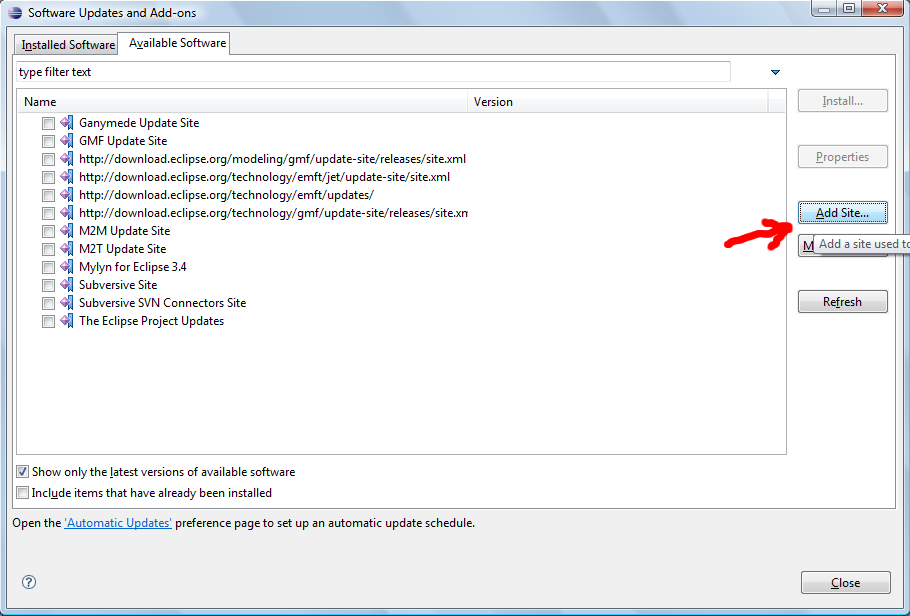
\includegraphics[width=1.0\linewidth]{figures/updateSite01}
	\caption{Adding an Eclipse Update Site.}
	\label{pic:updateSite01}
\end{figure}

Enter the path

\reference{http://dresden-ocl.svn.sourceforge.net/svnroot/dresden-ocl/trunk/ocl20forEclipse/\linebreak[0]updatesite/tudresden.ocl20.updatesite\_1.2.0}

and press the \eclipse{OK} button (see figure \ref{pic:updateSite02}). If an error occurs, please make sure, that you use \reference{http} instead of \reference{https}.

\begin{figure}[!htbp]
	\centering
	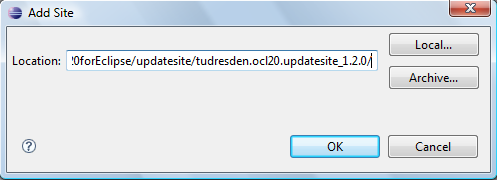
\includegraphics[width=0.7\linewidth]{figures/updateSite02}
	\caption{Adding the Dresden OCL2 for Eclipse Update Site.}
	\label{pic:updateSite02}
\end{figure}

Now you can select the features of \keyword{Dresden OCL2 for Eclipse} which you want to install. Select them and click on the \eclipse{Install ...} button (see figure \ref{pic:updateSite03}). An otherview about all features of \keyword{Dresden OCL2 for Eclipse} can be found in table \ref{ab:plugins}. Follow the wizard and agree with the user license. Then the Toolkit will be installed. Afterwords, you should restart your \keyword{Eclipse} application to finish the installation.

\begin{figure}[!htbp]
	\centering
	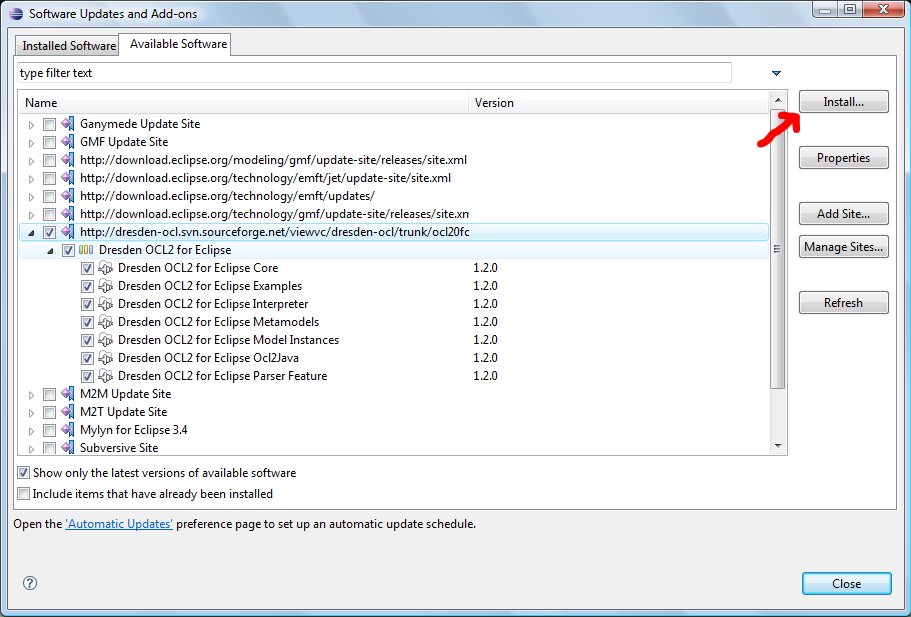
\includegraphics[width=1.0\linewidth]{figures/updateSite03}
	\caption{Selecting features of Dresden OCL2 for Eclipse.}
	\label{pic:updateSite03}
\end{figure}
	
	
	
\section{Importing Dresden OCL2 for Eclipse from the SVN}

To use \keyword{Dresden OCL2 for Eclipse} by checking out the source code from the SVN you need to install a SVN client. In the following the use the \keyword{Eclipse Subversive} plug-in and at least one of the \keyword{SVN Connectors} available at \cite{WWW:eclipseSubversive}.

After installing \keyword{Eclipse Subversive}, a new \keyword{Eclispe perspective} for access to \keyword{SVN} should exist. The perspective can be opened via the menu \eclipse{Window > Open Perpective > Other... > SVN Repository Exploring}. In the view \eclipse{SVN Repositories} you can add a new repository (see figure \ref{pic:SVN}) using the URL 

\begin{center}
\reference{https://dresden-ocl.svn.sourceforge.net/svnroot/dresden-ocl/}
\end{center}

After pressing the \eclipse{Finish} button the SVN repository root should the visible in the \eclipse{SVN Repositories} view. To checkout the plug-ins, you now select them in the repository directory \reference{trunk/ocl20forEclipse/eclipse} and use the \eclipse{Checkout...} function in the context menu (see figure \ref{pic:Checkout}).
	
\begin{figure}[!htbp]
	\centering
	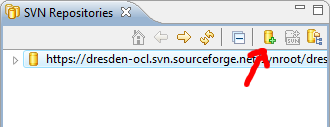
\includegraphics[width=0.5\linewidth]{figures/SVN}
	\caption{Adding an SVN repository.}
	\label{pic:SVN}
\end{figure}
	
\begin{figure}[!htbp]
	\centering
	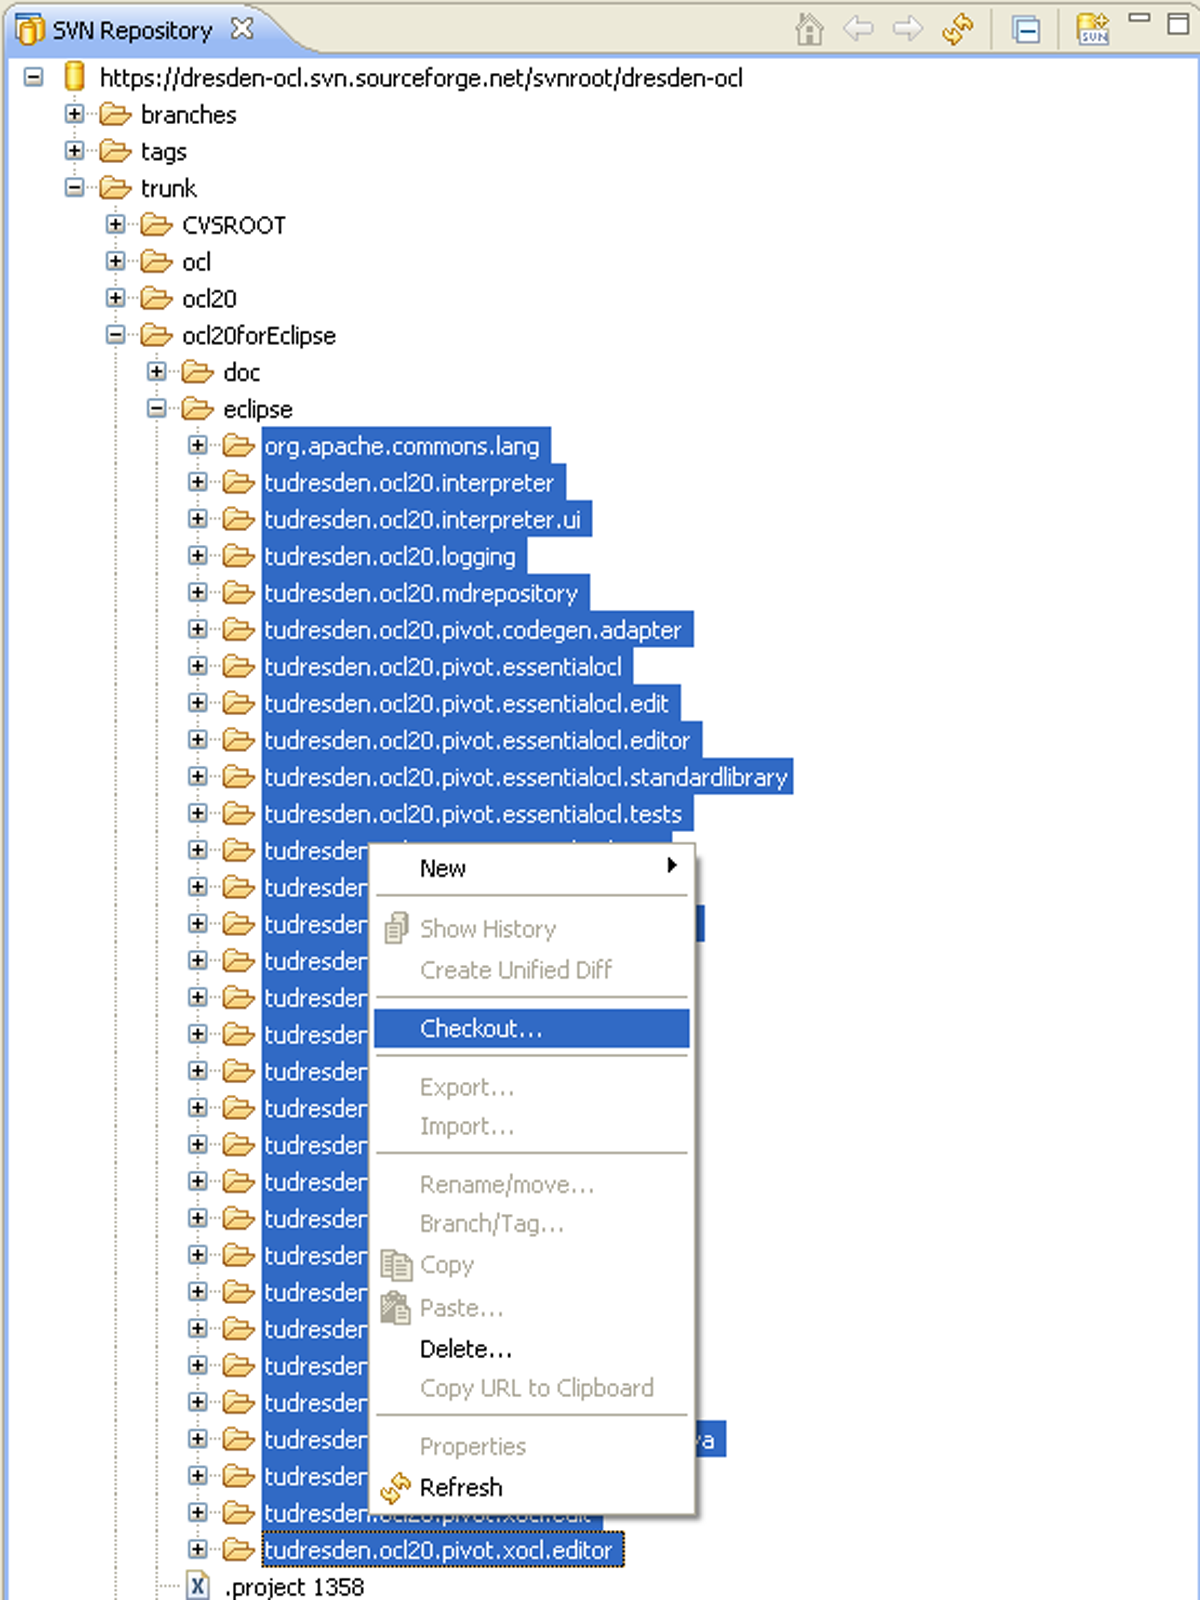
\includegraphics[width=0.5\linewidth]{figures/Checkout}
	\caption{Checkout of the Dresden OCL2 Toolkit plug-in projects.}
	\label{pic:Checkout}
\end{figure}


\section{Which Plug-ins do I need at least?}

An often asked question is ``Which plug-ins are at least required to run \keyword{Dresden OCL2 for Eclipse}?'' Well, the answer is: ``That depends.''. 

That depends on the things you want to do with \keyword{Dresden OCL2 for Eclipse}. Table \ref{tab:plugins} shows a list of the current plug-ins of \keyword{Dresden OCL2 for Eclipse}. Which are related to different features. You should install at least the \keyword{Core} feature, at least one of the \keyword{Metamodels}, and the \keyword{Parser} feature. The \keyword{Interpreter} and \keyword{OCL2Java} features are only required if you want to interpret constraints or to generate code. If you import or interpret modelinstances, you need to install the \keyword{Model Instances} feature as well. The examples of the \keyword{Example} feature are only required to run the examples provided in the tutorials available at \cite{WWW:toolkit}. This tutorial recommends to first install all provided features.
		


\section{Building the OCL2 Parser}
	
If you decided to run \keyword{Dresden OCL2 for Eclipse} as source code plug-ins from an \keyword{Eclipse} workspace, you need to build the \keyword{OCL2 Parser} via an \keyword{Ant} build script. If you installed the Toolkit using the update site, you can skip this section of the tutorial.
  
To build the \keyword{OCL2 Parser} select the file \reference{build.xml} in the project \reference{tudresden.\linebreak[0]ocl20.pivot.ocl2parser} and open the context menu via a right mouse click. Select the function \eclipse{Run As ... > Ant Build ...} (see figure \ref{pic:Build}).

\begin{figure}[!htbp]
	\centering
	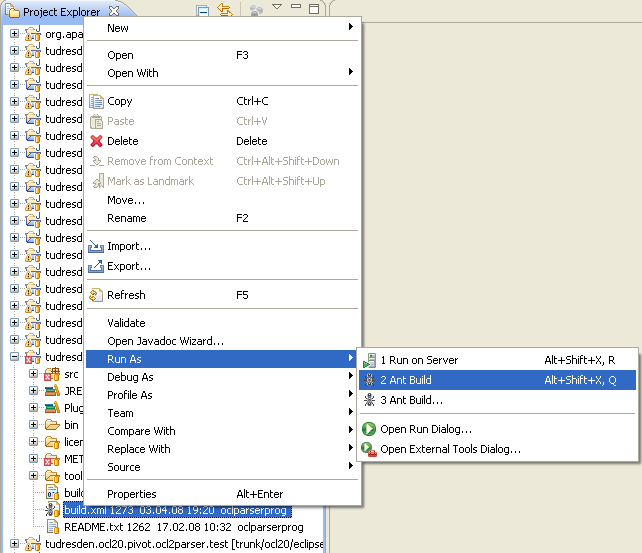
\includegraphics[width=0.8\linewidth]{figures/Build}
	\caption{Executing the OCL2 parser build script.}
	\label{pic:Build}
\end{figure}
	
A new window should open. Select in the sub menu \keyword{JRE} the check box \keyword{Run in the same JRE as the workspace} and click on the button \keyword{OK} (see figure \ref{pic:AntConfig}). Afterwards the \keyword{Ant} parser should be generated without errors. If an error like \eclipse{Unable to find javac compiler.} occurs, you might be trying to run the \keyword{Ant} script with an \keyword{Java Runtime Environment} instead of the \keyword{Java Development Kit} (For errors like) use the \eclipse{Installed JREs...} button in the same window to select a \keyword{JDK} instead.
	
\begin{figure}[!htbp]
	\centering
	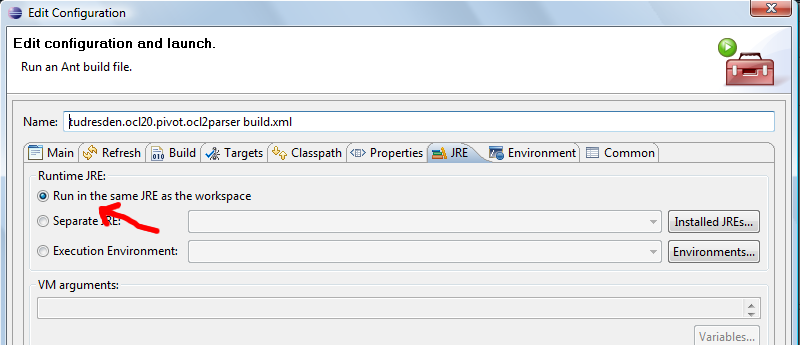
\includegraphics[width=1.0\linewidth]{figures/AntConfig}
	\caption{Settings of the JRE for the Ant build script.}
	\label{pic:AntConfig}
\end{figure}
	
After executing the build script successfully you need to update the projects in your workspace. Update the project \reference{tudresden.ocl20.pivot.oclparser} via context menu (\eclipse{Refresh}, see figure \ref{pic:Refresh}).

\begin{figure}[!htbp]
	\centering
	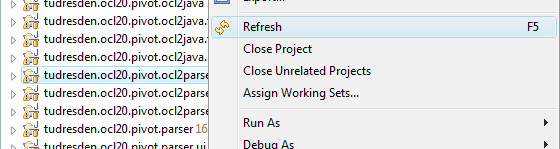
\includegraphics[width=0.8\linewidth]{figures/Refresh}
	\caption{Refreshing the project ``tudresden.ocl20.pivot.oclparser''.}
	\label{pic:Refresh}
\end{figure}
	
Additionally you need to recompile all depending projects. Select the function \eclipse{Project > Clean... > Clean all projects} in the \keyword{Eclipse} menu to clean all projects. Now all the projects should not contain errors anymore and should be executable.



	
\chapter{Loading Models, Model Instances and OCL Constraints}

If you installed the \keyword{Dresden OCL2 for Eclipse} using the update site, you can execute the toolkit by re-starting your \keyword{Eclipse} distribution. If you imported the Toolkit as source code plug-ins into an \keyword{Eclipse} workspace, you have to start a new \keyword{Eclipse} instance. You can start a new instance via the menu \eclipse{Run > Run As > Eclipse Application}. If the menu \eclipse{Eclipse Application} is not available or disabled you need to select one of the plug-ins of the toolkit first.



\section{The Simple Example}

This tutorial explains \keyword{Dresden OCL2 for Eclipse} using the \keyword{Simple Example} which is located in the plug-in package \reference{tudresden.ocl20.pivot.examples.\linebreak[0]simple}. Figure \ref{pic:Simple} shows the class diagram of the \keyword{Simple Example}.

\begin{figure}[!htbp]
	\centering
	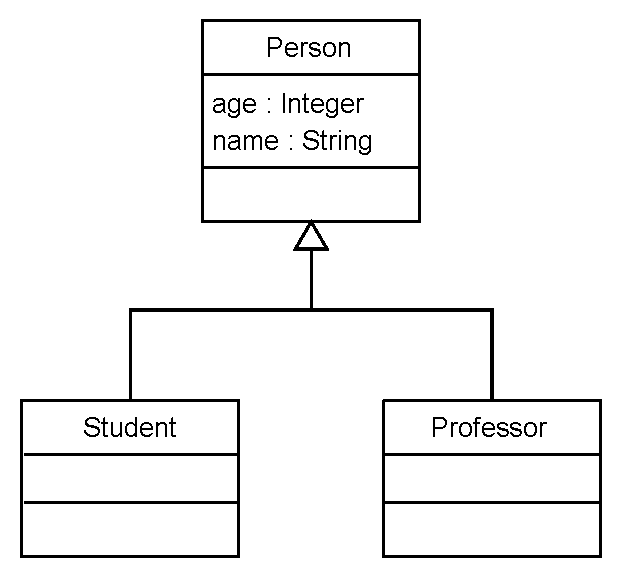
\includegraphics[width=0.5\linewidth]{figures/simpleExample}
	\caption{The class diagram described by the simple example model.}
	\label{pic:Simple}
\end{figure}

\keyword{Dresden OCL2 for Eclipse} provides more examples than the \keyword{Simple Example}. The different examples use different meta models which is possible with the \textit{Pivot Model} architecture of the Toolkit. An overview about all examples provided with \keyword{Dresden OCL2 for Eclipse} can be found in \cite{tut:examples}. The \keyword{Simple example} can be used with two different meta models. These are \keyword{UML 2.0} (based on \keyword{Eclipse MDT UML2}) and \keyword{EMF Ecore}.
	

	
\section{Loading a Domain-Specific Model}
	
After starting \keyword{Eclipse} you have to load a model into the toolkit. If the plug-ins of \keyword{Dresden OCL2 for Eclipse} have been installed using the update site, the \keyword{Simple Example} plug-in has to be imported into the \keyword{Workspace} first. Create a new Java project into your \keyword{Workspace} and select the \keyword{import wizard} \eclipse{General > Archive File}. In the following window select the \eclipse{plugins} directory in your \keyword{Eclipse} root folder, select the archive \reference{tudresden.ocl20.pivot.examples.\linebreak[0]simple\_1.0.0.jar} and click the \eclipse{Finish} button.

Now you can load a model. Select the menu option \eclipse{Dresden OCL2 > Load Model}. In the opened wizard you have to select a model file and a meta model for the model (see figure \ref{pic:LoadModel}). Click the button \eclipse{Browse Workspace...} and select the file \reference{model/simple.uml} inside the \keyword{Simple Example Project}. Then select the meta model \keyword{UML2} and press the button \eclipse{Finish}.

\begin{figure}[!htbp]
	\centering
	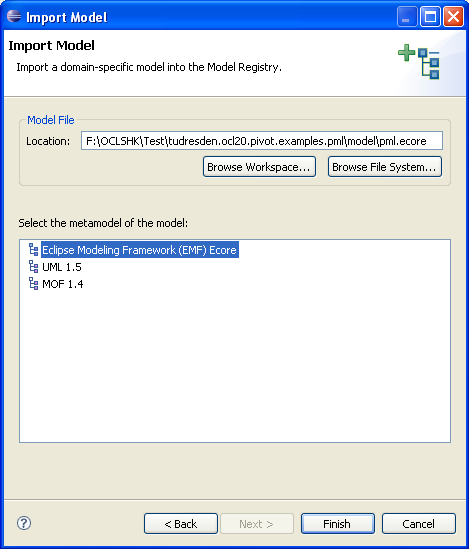
\includegraphics[width=0.8\linewidth]{figures/LoadModel}
	\caption{Loading a domain specific model.}
	\label{pic:LoadModel}
\end{figure}
	
Figure \ref{pic:MoBrOE} shows the loaded \keyword{Simple} model, which uses \keyword{UML2} as its meta model. Via the menu button of the \eclipse{Model Browser} (the little triangle in the right top corner) you can switch between different models (see figure \ref{pic:SwitchModel}).
	
\begin{figure}[!htbp]
	\centering
	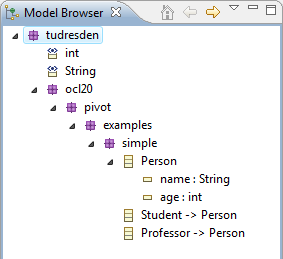
\includegraphics[width=0.5\linewidth]{figures/MoBrOE}
	\caption{The loaded Simple Example model in the model browser.}
	\label{pic:MoBrOE}
\end{figure}

\begin{figure}[!htbp]
	\centering
	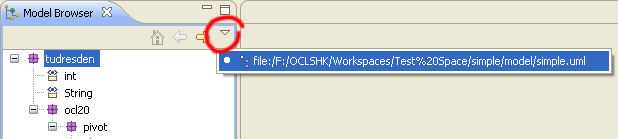
\includegraphics[width=0.6\linewidth]{figures/SwitchModel}
	\caption{You can switch between different models using the little triangle.}
	\label{pic:SwitchModel}
\end{figure}

	
\section{Loading a Model Instance}
	
After loading the model, you can load a \keyword{model instance} using another \keyword{wizard}. Use the menu option \eclipse{Dresden OCL2 > Load Model Instance}. In the opened wizard you have to select a model instance (in this tutorial we used the file \reference{bin/tudresden/ocl20/\linebreak[0]pivot/examples/ModelProviderClass.class} of the \keyword{Simple Example} a domain-specific model loaded before (see figure \ref{pic:LoadInstance}). Besides the model instance resource you have to select a model for which the model instance shall be loaded and the type of model instance you want to load (we want to load a \keyword{Java Instance}).

\begin{figure}[!htbp]
	\centering
	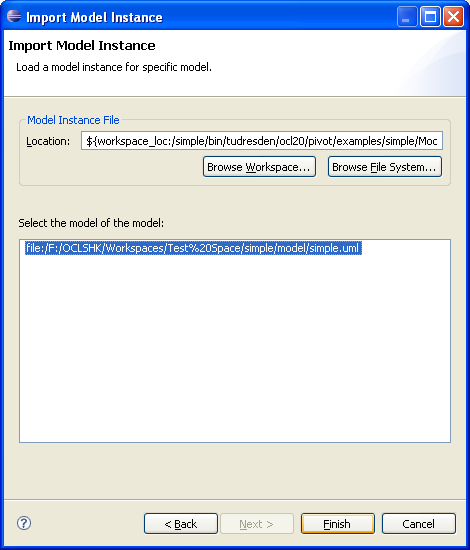
\includegraphics[width=0.8\linewidth]{figures/LoadInstance}
	\caption{Loading a simple model instance.}
	\label{pic:LoadInstance}
\end{figure}
	
Figure \ref{pic:MoInBr} shows the loaded model instance of the \keyword{Simple Example} model. Like in the model browser you can switch between different model instances. Note that the model instance browser only shows the model instances of the model actually selected in the model browser. By switching the domain specific model, you also switch the pool of model instances available in the model instance browser.

\begin{figure}[!htbp]
	\centering
	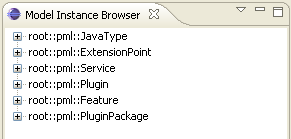
\includegraphics[width=0.5\linewidth]{figures/MoInBr}
	\caption{A simple model instance in the Model Instance Browser.}
	\label{pic:MoInBr}
\end{figure}

	

\section{Parsing OCL expressions}
	
Before you can interpret OCL constraints you have to load them like the domain-specific model and the model instance before. Use the menu option \eclipse{Dresden OCL2 > OCL Expressions} and select an OCL file (in this tutorial we used the OCL file \reference{constraints/invariants.ocl} of the \keyword{Simple Example}, see figure \ref{pic:LoadExpressions}). The constraints of the file \reference{constraints/invariants.ocl} are shown in listing \ref{list:invariants}.

\begin{figure}[!htbp]
	\centering
	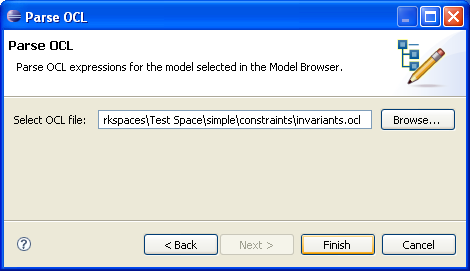
\includegraphics[width=0.8\linewidth]{figures/LoadExpressions}
	\caption{The import of OCL expressions.}
	\label{pic:LoadExpressions}
\end{figure}
	
\lstset{
  language=OCL
}
\begin{lstlisting}[caption={The invariants of the simple examples.}, captionpos=b, label=list:invariants, float]
package tudresden::ocl20::pivot::examples::simple

-- The age of Person can't be negative.
context Person
inv: age >= 0

-- Students should be 16 or older.
context Student
inv: age > 16

-- Proffesors should be at least 30.
context Professor
inv: not (age < 30)

endpackage
\end{lstlisting}

The expressions of the selected OCL file will be loaded into the actually selected model. Figure \ref{pic:MoBrME} shows the \reference{Model Browser} containing the model and the parsed expressions.
	
\begin{figure}[!htbp]
	\centering
	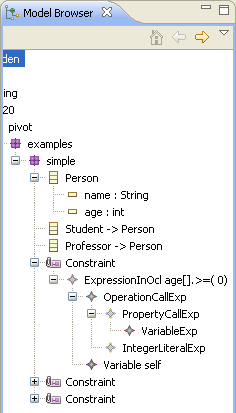
\includegraphics[width=0.5\linewidth]{figures/MoBrME}
	\caption{Parsed expressions and the model in the Model Browser.}
	\label{pic:MoBrME}
\end{figure}
	
	
	
	
\chapter{Conclusion}
  
This tutorial described how to use \keyword{Dresden OCL2 for Eclipse}. It explained how to install the Toolkit's plug-ins. Afterwards, the loading of domain-specific models, model instances and OCL constraints into the Toolkit has been explained.

Now, the imported models can be used to use the tools provided with \keyword{Dresden OCL2 for Eclipse}. For example you can use the \keyword{OCL2 Interpreter} of \keyword{Dresden OCL2 for Eclipse} to interpret OCL constraints for a given model and model instance or you can use the \keyword{OCL22Java Code Generator} to generate \keyword{AspectJ} code for a loaded model and OCL constraints. Tutorials how to use the OCL2 Interpreter and the other tools provided with \keyword{Dresden OCL2 for Eclipse} can be found at \cite{WWW:toolkit} in the \keyword{Dresden OCL2 for Eclipse > Usage} section.




\chapter{A Short Note about Logging}

\keyword{Dresden OCL2 for Eclipse} uses a \keyword{Log4j} logger to log method entries, exits and errors during the Toolkit's execution. If you run \keyword{Dresden OCL2 for Eclipse} as source code plug-ins from an \keyword{Eclipse} workspace, you might receive exceptions like

\begin{center}
\reference{log4j:ERROR Could not connect to remote log4j server at [localhost].}
\end{center}

 although the Toolkit works correctly. This is because the \keyword{Log4j} logger tries to sent the logged events to a server running at \reference{localhost}.

To solve this problem (if you want to) you have to install and setup a logging server at your computer. One logging server you might use is called \keyword{Chainsaw} and available at \cite{WWW:chainsaw}. If you start \keyword{Chainsaw}, set up a \keyword{SocketReceiver} at port \keyword{4445 (Old Style/Standard Chainsaw Port)} (see figure \ref{pic:chainsaw}).

\begin{figure}[!htbp]
	\centering
	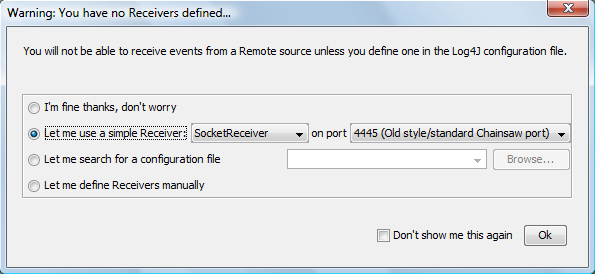
\includegraphics[width=0.8\linewidth]{figures/chainsaw}
	\caption{Setting up a simple SocketReceiver in Chainsaw.}
	\label{pic:chainsaw}
\end{figure}

	


\appendix

\chapter{Tables}

\begin{table}
\begin{tabular}{|p{7cm}|p{7cm}|}
    \hline
    \textbf{Software} & \textbf{Available at} \\
    \hline
    Eclipse 3.4.x & http://www.eclipse.org/ \\
    \hline
    Eclipse Modeling Framework (EMF) & http://www.eclipse.org/modeling/emf/ \\
    \hline
    Eclipse Model Development Tools (MDT) (only with the UML2.0 meta model) & http://www.eclipse.org/modeling/mdt/ \\
    \hline
    Eclipse Plug-in Development Environment (only to run the toolkit using the source code distribution) & http://www.eclipse.org/pde/ \\
    \hline
\end{tabular}
\caption{Software needed to run Dresden OCL2 for Eclipse (\textbf{If not using the Eclipse MDT Distribution)}.}
\label{tab:software}
\end{table}

\begin{table}
\begin{tabular}[h]{|p{4cm}|p{10cm}|}
    \hline
    \textbf{Feature} & \textbf{Plug-ins} \\
    \hline

    \textbf{Core} & 
    \textbf{Required:}\newline
    org.apache.commons.lang\newline
    tudresden.ocl20.pivot.logging\newline
    tudresden.ocl20.pivot.essentialocl\newline
    tudresden.ocl20.pivot.essentialcol.edit\newline
    tudresden.ocl20.pivot.essentialocl.editor\newline
    tudresden.ocl20.pivot.essentialocl.standardlibrary\newline
    tudresden.ocl20.pivot.modelbus\newline
    tudresden.ocl20.pivot.modelbus.ui\newline
    tudresden.ocl20.pivot.pivotmodel\newline
    tudresden.ocl20.pivot.pivotmodel.edit\newline
    tudresden.ocl20.pivot.standardlibrary\newline\newline
    \textbf{Optional:}\newline
    tudresden.ocl20.pivot.essentialocl.tests\newline
    tudresden.ocl20.pivot.pivotmodel.tests\\
    \hline

    \textbf{Examples} &
    \textbf{Optional:}\newline
    tudresden.ocl20.pivot.examples.living\newline
    tudresden.ocl20.pivot.examples.pml\newline
    tudresden.ocl20.pivot.examples.royalandloyal\newline
    tudresden.ocl20.pivot.examples.royalandloyal.constraints\newline
    tudresden.ocl20.pivot.examples.simple\newline
    tudresden.ocl20.pivot.examples.simple.constraints\\
    \hline

    \textbf{Interpreter} &
    \textbf{Required (for interpretation):}\newline
    tudresden.ocl20.interpreter\newline
    tudresden.ocl20.interpreter.ui\newline\newline
    \textbf{Optional:}\newline
    tudresden.ocl20.interpreter.test\\
    \hline
 
    \textbf{Metamodels} &
    \textbf{Required (at least one of the following):}\newline
    tudresden.ocl20.pivot.metamodels.ecore\newline
    tudresden.ocl20.pivot.metamodels.uml2\\
    \hline
 
    \textbf{Model Instances} &
    \textbf{Required (at least one of the following for interpretation):}\newline
    tudresden.ocl20.pivot.modelinstancetype.ecore\newline
    tudresden.ocl20.pivot.modelinstancetype.java\\
    \hline
 
    \textbf{Ocl2Java} &
    \textbf{Required (for code generation):}\newline
    tudresden.ocl20.pivot.ocl2java\newline
    tudresden.ocl20.pivot.ocl2java.ui\newline\newline
    \textbf{Optional (eventually for code execution):}\newline
    tudresden.ocl20.pivot.ocl2java.types\newline\newline
    \textbf{Optional:}\newline
    tudresden.ocl20.pivot.ocl2java.test\\
    \hline

    Dresden OCL2 for Eclipse Parser Feature &
    \textbf{Required:}\newline
    tudresden.ocl20.pivot.ocl2parser\newline
    tudresden.ocl20.pivot.parser\newline
    tudresden.ocl20.pivot.parser.ui\newline\newline
    \textbf{Optional:}\newline
    tudresden.ocl20.pivot.ocl2parser.test\\
    \hline
\end{tabular}
\caption{The plug-ins of Dresden OCL2 for Eclipse related to their feature.}
\label{tab:plugins}
\end{table}




\listoffigures
\addcontentsline{toc}{chapter}{List of Figures}




\bibliographystyle{alphadin}
\bibliography{tutorial}
% Literaturliste in Inhalt aufnehmen.
\addcontentsline{toc}{chapter}{References}




\end{document}